\section{图片}
\label{sec:00-pictures}

\subsection{一张图}

写法：

\begin{lstlisting}[language=TeX]
\begin{figure}[htbp]
\centering
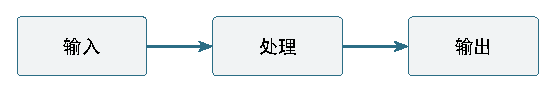
\includegraphics[width=.7\linewidth]{figures/05-pictures/demo-flow}
\caption{数据流示意}
\label{fig:00-flow}
\end{figure}
\end{lstlisting}

效果：

\begin{figure}[htbp]
\centering
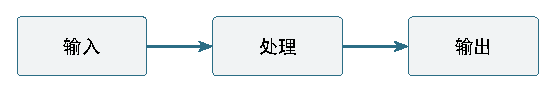
\includegraphics[width=.7\linewidth]{figures/05-pictures/demo-flow}
\caption{数据流示意}
\label{fig:00-flow}
\end{figure}

宽度用 \verb|width=.7\linewidth| 表示"占版心的 70\%"；写成
\verb|width=\linewidth| 就是占满。加 \verb|keepaspectratio| 可以保证不变形
（默认按比例缩放，通常不需要）。

\subsection{两张图并排}

并排用 \texttt{minipage} 左右各占一半，各自带图题：

\begin{lstlisting}[language=TeX]
\begin{figure}[htbp]
\centering
\begin{minipage}{.48\linewidth}
  \centering
  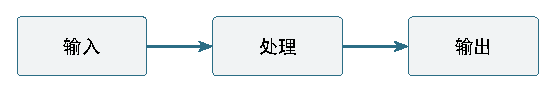
\includegraphics[width=\linewidth]{figures/05-pictures/demo-flow}
  \caption{左图：数据流}
  \label{fig:00-left}
\end{minipage}\hfill
\begin{minipage}{.48\linewidth}
  \centering
  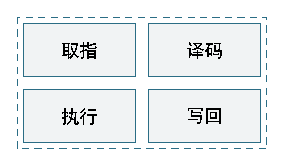
\includegraphics[width=\linewidth]{figures/05-pictures/demo-blocks}
  \caption{右图：阶段划分}
  \label{fig:00-right}
\end{minipage}
\end{figure}
\end{lstlisting}

效果：

\begin{figure}[htbp]
\centering
\begin{minipage}{.48\linewidth}
  \centering
  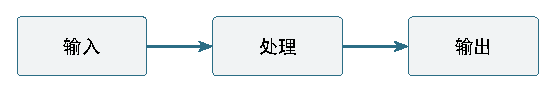
\includegraphics[width=\linewidth]{figures/05-pictures/demo-flow}
  \caption{左图：数据流}
  \label{fig:00-left}
\end{minipage}\hfill
\begin{minipage}{.48\linewidth}
  \centering
  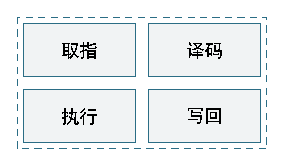
\includegraphics[width=\linewidth]{figures/05-pictures/demo-blocks}
  \caption{右图：阶段划分}
  \label{fig:00-right}
\end{minipage}
\end{figure}

左图是\cref{fig:00-left}，右图是\cref{fig:00-right}——引用时自动带编号。

注意这两张图不一定排在这一段旁边：\textbf{图和表都会浮动}，会被排到页面上更合适的
位置。正因为如此，正文里要写"见\cref{fig:00-left}"，不要写"如下图"。

\subsection{直接用代码画的图}

简单的框图和时序示意其实不必存成图片文件，用 TikZ 直接画在正文里，改起来更快：

\begin{lstlisting}[language=TeX]
\begin{tikzpicture}[box/.style={draw=Accent,fill=Brand!6,rounded corners=2pt,
  minimum width=20mm,minimum height=9mm,align=center,font=\sffamily\small}]
\node[box] (a) {取指};
\node[box,right=8mm of a] (b) {执行};
\draw[->,thick,Accent] (a) -- (b);
\end{tikzpicture}
\end{lstlisting}

效果：

\begin{center}
\begin{tikzpicture}[box/.style={draw=Accent,fill=Brand!6,rounded corners=2pt,
  minimum width=20mm,minimum height=9mm,align=center,font=\sffamily\small}]
\node[box] (a) {取指};
\node[box,right=8mm of a] (b) {执行};
\draw[->,thick,Accent] (a) -- (b);
\end{tikzpicture}
\end{center}

\KeyPoint{选哪种}{需要精确标注的电路图、结构图，用 TikZ 画（矢量、可改）；
截图、相机拍的照片、扫描件，存成图片文件放本章的 \texttt{figures/} 下。
图片文件的命名用小写英文加连字符，例如 \texttt{pipeline-hazard.pdf}。}
